\documentclass[12pt]{article}

% Information Geometry (Springer) formatting
\usepackage[margin=1in]{geometry}
\usepackage{amsmath,amssymb,amsthm}
\usepackage{graphicx}
\usepackage{hyperref}
\usepackage[numbers,square]{natbib}
\usepackage{booktabs}
\usepackage{caption}
\usepackage{subcaption}

% Theorem environments
\newtheorem{theorem}{Theorem}
\newtheorem{lemma}[theorem]{Lemma}
\newtheorem{proposition}[theorem]{Proposition}
\newtheorem{corollary}[theorem]{Corollary}
\newtheorem{definition}[theorem]{Definition}
\newtheorem{remark}[theorem]{Remark}
\newtheorem{example}[theorem]{Example}

% Custom commands
\newcommand{\R}{\mathbb{R}}
\newcommand{\M}{\mathcal{M}}
\newcommand{\F}{\mathcal{F}}
\newcommand{\T}{\mathcal{T}}
\newcommand{\pr}{\text{PR}}

\title{Minimal Embedding Dimension for Self-Intersection-Free \\
Recurrent Processes on Statistical Manifolds}

\author{Ian Todd\\
Sydney Medical School, University of Sydney\\
\texttt{itod2305@uni.sydney.edu.au}}

\date{}

\begin{document}

\maketitle

\begin{abstract}
We study the problem of embedding recurrent processes on statistical manifolds into Euclidean spaces of minimal dimension while preserving temporal distinctness. A \emph{self-intersection} occurs when two temporally distinct points of a trajectory are mapped to the same point in the embedding space. We show that for a class of cyclic processes with strictly monotone meta-time---including recurrent neural dynamics, biological oscillators, and symbolic state transitions---any continuous \emph{phase-preserving} embedding into $\R^2$ (i.e., one that maps the cycle to a simple closed curve, with image depending only on phase and not on meta-time) necessarily produces self-intersections, whereas self-intersection-free embeddings into $\R^3$ always exist. This establishes $k=3$ as a critical dimension threshold for phase-preserving representations of recurrent processes: $k \leq 2$ forces categorical discretization through unavoidable state conflation, while $k \geq 3$ preserves the continuous structure of temporal dynamics. We interpret this result in terms of metric degeneracy under dimensional collapse: the Fisher information metric loses rank when the meta-time coordinate is projected out.
\end{abstract}

\noindent\textbf{Keywords:} information geometry, dimensional reduction, statistical manifolds, embedding dimension, recurrent dynamics

\section{Introduction}

Information geometry provides a natural framework for studying inference and decision-making, endowing families of probability distributions with Riemannian structure via the Fisher information metric \citep{amari2016information,rao1945information}. In this framework, learning and reasoning correspond to trajectories on statistical manifolds, and the geometry of these manifolds constrains what inferences are possible.

A fundamental question arises when we consider \emph{dimensional collapse}: what happens when a high-dimensional statistical manifold is projected onto a lower-dimensional subspace? The notion of dimensional collapse has geometric precedent in Cheeger-Gromov collapsing theory \citep{cheeger1986collapsing}, where Riemannian manifolds collapse under curvature bounds; our notion differs in that collapse occurs through projection rather than diameter shrinkage. This situation is ubiquitous in practice---from rate-distortion theory \citep{shannon1959coding} and the information bottleneck \citep{tishby2000information} to low-dimensional neural representations \citep{gallego2017neural}.

In this paper, we focus on a specific aspect of dimensional collapse: the emergence of \emph{self-intersections} between temporally distinct states. When a trajectory $\gamma(t)$ on a statistical manifold $\M$ is projected to a lower-dimensional space via a map $\pi_k: \M \to \R^k$, distinct times $t_1 \neq t_2$ may be mapped to the same point: $\pi_k(\gamma(t_1)) = \pi_k(\gamma(t_2))$. Such self-intersections destroy temporal information and force the system into a discrete, categorical regime.

The question of minimal embedding dimension has a rich history in differential topology, beginning with Whitney's embedding theorem: Whitney \citep{whitney1936manifolds} showed that any smooth $n$-manifold can be embedded in $\R^{2n+1}$, and later \citep{whitney1944selfintersections} sharpened this to $\R^{2n}$. For dynamical systems, Takens' embedding theorem \citep{takens1981detecting} provides conditions under which time-delay embeddings reconstruct attractor geometry. Our contribution is to apply these ideas in the information-geometric setting, asking specifically: what is the minimal dimension required to embed \emph{recurrent processes with monotone meta-time} without self-intersection?

Our main results establish that:
\begin{enumerate}
    \item For cyclic processes with monotone meta-time, self-intersections are structurally unavoidable in $\R^2$ under \emph{phase-preserving} embeddings---those that map the cycle to a simple closed curve with image depending only on phase, not on meta-time. (Embeddings that encode meta-time in the radial coordinate, such as spirals, can avoid self-intersections but violate this constraint.)
    \item Self-intersection-free embeddings into $\R^3$ always exist for these processes.
    \item The dimension $k = 3$ is therefore a \emph{critical threshold} for phase-preserving representations: categorical below, continuous above.
\end{enumerate}

\textbf{Why phase-preservation is not arbitrary.} The phase-preserving constraint arises naturally in several settings: (i) when a 2D representation is required to depict the \emph{cyclic structure} as a closed curve (e.g., limit cycles, phase diagrams, cyclic state machines); (ii) when the representation must be equivariant or invariant under meta-time reparametrization---so that ``where in the cycle'' is displayed, but ``which traversal'' is not; (iii) when bounded spatial representations are required, ruling out unbounded spirals. The theorem's content is that under these natural constraints, self-intersections are unavoidable. The proof is elementary, but the result identifies a sharp geometric threshold with implications for when discrete/symbolic representations must emerge from continuous dynamics.

This result connects to classical dynamical systems theory: the Poincar\'e-Bendixson theorem \citep{poincare1881memoire,bendixson1901courbes,guckenheimer1983nonlinear} states that continuous flows in $\R^2$ cannot exhibit chaotic behavior---only fixed points and limit cycles are possible. Our work provides an information-geometric analog: $k=2$ constrains representable dynamics to categorical structures, while $k \geq 3$ permits richer process-oriented dynamics.

\textbf{Companion paper.} This paper establishes a specific phenomenon; a companion paper \citep{todd2025quotient} develops the general quotient-geometric framework that makes the phenomenon inevitable. In that framework, collapse maps induce vertical/horizontal distributions ($\mathcal{V} = \ker(d\pi)$, $\mathcal{H} = \mathcal{V}^\perp$), the Fisher metric descends to a quotient under bundle-like conditions, and covering numbers $N(\varepsilon) \sim \varepsilon^{-r}$ quantify distinguishability at rank $r$. The $k = 3$ threshold established here corresponds to a transition from scaling exponent $r = 1$ (phase-only) to $r = 2$ (phase-and-time)---see the companion paper for the explicit connection.

\section{Preliminaries}

\subsection{Statistical Manifolds and the Fisher Metric}

Let $\M = \{p_\theta : \theta \in \Theta\}$ be a parametric family of probability distributions on a sample space $\mathcal{X}$, where $\Theta \subseteq \R^n$ is an open subset. Under regularity conditions, $\M$ carries the structure of a Riemannian manifold with the Fisher information metric \citep{amari2000methods,fisher1925theory}:
\begin{equation}
    g_{ij}(\theta) = \mathbb{E}_{p_\theta}\left[\frac{\partial \log p_\theta}{\partial \theta^i} \frac{\partial \log p_\theta}{\partial \theta^j}\right].
\end{equation}

The Fisher metric captures the local distinguishability of nearby distributions: the geodesic distance between $p_\theta$ and $p_{\theta + d\theta}$ measures how statistically distinguishable they are.

\subsection{Dimensional Collapse Maps}

\begin{definition}[Collapse Map]\label{def:collapse}
A \emph{dimensional collapse map} is a smooth map $\pi_k: \M \to \R^k$ where $k < \dim(\M)$. Given $\pi_k$, the \emph{observable} (or \emph{effective}) Fisher information is obtained by restricting attention to directions detectable through $d\pi_k$. In general this yields a rank-deficient semi-metric on $\M$; a full quotient metric on the image space $\M/{\sim_\pi}$ requires additional regularity conditions (see the companion paper for the general quotient-geometric framework).
\end{definition}

When $k < \dim(\M)$, the observable information generically has rank less than $\dim(\M)$: some directions in parameter space become indistinguishable after projection. Collapse maps relate to the theory of sufficient statistics in information geometry \citep{ay2017information}, where projections that preserve Fisher information define sufficient statistics; our collapse maps are precisely those that fail this criterion. This phenomenon is also connected to singularities in statistical learning theory \citep{watanabe2009algebraic}.

\subsection{Recurrent Processes and Trajectories}

\begin{definition}[Recurrent Process]
A \emph{recurrent process} on $\M$ is a continuous curve $\gamma: [0, T] \to \M$ representing the evolution of a belief state or inference trajectory.
\end{definition}

\begin{definition}[Cyclic Process with Monotone Meta-Time]\label{def:cyclic}
A recurrent process $\gamma$ is \emph{cyclic with monotone meta-time} if:
\begin{enumerate}
    \item There exists a ``phase coordinate'' projection $\varphi: \M \to S^1$ such that $\varphi \circ \gamma$ covers the circle $n \geq 2$ times. We identify $S^1 \cong \R/\mathbb{Z}$ and write $\varphi \in [0,1)$; the expression $\cos(2\pi\varphi)$ then gives the standard embedding of the circle in $\R^2$.
    \item The process encodes a strictly monotone ``meta-time'' variable $\tau: [0,T] \to \R$ with $\tau'(t) > 0$ for all $t$.
\end{enumerate}
\end{definition}

\begin{example}[Recurrent Systems]
This class includes:
\begin{itemize}
    \item \textbf{Biological oscillators:} Neural limit cycles, circadian rhythms, cardiac pacemakers.
    \item \textbf{Recurrent neural networks:} Hidden state trajectories in RNNs processing sequential data.
    \item \textbf{Logical paradoxes:} The Liar's paradox (``This statement is false'') oscillates between TRUE and FALSE, with each cycle occurring at a distinct meta-time.
\end{itemize}
\end{example}

\begin{lemma}[Intrinsic Cylinder Structure]\label{lem:cylinder}
A cyclic process with monotone meta-time (Definition~\ref{def:cyclic}) carries an intrinsic \emph{cylinder structure}. Specifically, the map
\begin{equation}
    \Phi: [0,T] \to S^1 \times \R, \quad \Phi(t) = (\varphi(\gamma(t)), \tau(t))
\end{equation}
embeds the trajectory into the cylinder $S^1 \times \R$, where:
\begin{itemize}
    \item The $S^1$ factor encodes the cyclic phase coordinate $\varphi$.
    \item The $\R$ factor encodes the strictly monotone meta-time $\tau$.
\end{itemize}
Since $\tau$ is strictly monotone, $\Phi$ is injective. The minimal embedding problem thus reduces to: \emph{what is the smallest $k$ such that this cylinder-structured trajectory admits a phase-preserving embedding into $\R^k$ without self-intersection?}
\end{lemma}

\begin{proof}
Injectivity of $\Phi$ follows from strict monotonicity of $\tau$: if $\Phi(t_1) = \Phi(t_2)$, then $\tau(t_1) = \tau(t_2)$, which implies $t_1 = t_2$ by monotonicity.
\end{proof}

\begin{remark}[Topological Note]
The cylinder $S^1 \times \R$ \emph{can} be embedded in $\R^2$---for example, as a spiral via $(\varphi, \tau) \mapsto (e^\tau \cos\varphi, e^\tau \sin\varphi)$. The obstruction in Theorem~\ref{thm:main} arises not from the cylinder topology alone, but from the \emph{phase-preserving} constraint (Eq.~\ref{eq:phase-preserving}), which requires the image to depend only on phase $\varphi$, effectively collapsing the cylinder fibers onto a circle. Spiral embeddings violate this constraint by encoding meta-time in the radial coordinate.
\end{remark}

\subsection{Self-Intersections and Injectivity}

\begin{definition}[Self-Intersection]\label{def:intersection}
Given a collapse map $\pi_k$ and a trajectory $\gamma: [0,T] \to \M$, a \emph{self-intersection} occurs when there exist distinct times $t_1, t_2 \in [0,T]$ with $t_1 \neq t_2$ such that:
\begin{equation}
    \pi_k(\gamma(t_1)) = \pi_k(\gamma(t_2)).
\end{equation}
Equivalently, the composed map $\pi_k \circ \gamma: [0,T] \to \R^k$ fails to be injective.
\end{definition}

\begin{definition}[Self-Intersection-Free Embedding]\label{def:sif}
A collapse map $\pi_k$ is \emph{self-intersection-free} for trajectory $\gamma$ if $\pi_k \circ \gamma$ is injective, i.e.,
\[
t_1 \neq t_2 \implies \pi_k(\gamma(t_1)) \neq \pi_k(\gamma(t_2)).
\]
\end{definition}

\begin{remark}[Collision Measure]
For numerical analysis, we count the \emph{collision set}:
\begin{equation}
    \mathcal{C}(\pi_k, \gamma) = \{(t_1, t_2) \in [0,T]^2 : t_1 < t_2 \text{ and } \|\pi_k(\gamma(t_1)) - \pi_k(\gamma(t_2))\| < \varepsilon\}
\end{equation}
for small $\varepsilon > 0$. The embedding is self-intersection-free if and only if $\mathcal{C} = \emptyset$ in the limit $\varepsilon \to 0$. In practice, we report $|\mathcal{C}|$ for finite $\varepsilon$ as an approximate collision count.
\end{remark}

\section{Main Results}

\subsection{The Minimal Embedding Theorem}

Our main result characterizes when self-intersection-free embeddings exist:

\begin{theorem}[Minimal Embedding Dimension]\label{thm:main}
Let $\gamma: [0, T] \to \M$ be a cyclic process with monotone meta-time as in Definition~\ref{def:cyclic}, with phase projection $\varphi: \M \to S^1$ and meta-time $\tau$. Let $K = \gamma([0,T]) \subset \M$ denote the trajectory image. Then:
\begin{enumerate}
    \item[(i)] \textbf{(Non-existence in $\R^2$)} Any continuous \emph{phase-preserving} map $\pi_2: K \to \R^2$---meaning $\pi_2$ factors through phase:
    \begin{equation}\label{eq:phase-preserving}
        \pi_2|_K = f \circ \varphi|_K
    \end{equation}
    for some continuous $f: S^1 \to \R^2$---necessarily has self-intersections: $\pi_2 \circ \gamma$ is not injective.
    \item[(ii)] \textbf{(Existence in $\R^3$)} There exists a continuous $\pi_3: K \to \R^3$ such that $\pi_3 \circ \gamma$ is injective (self-intersection-free).
\end{enumerate}
\end{theorem}

\begin{remark}[Why Phase-Preservation Matters]
The phase-preserving condition \eqref{eq:phase-preserving} excludes embeddings that use ``hidden dimensions'' to encode meta-time. For instance, a spiral $(\cos\varphi, \sin\varphi, r(\tau))$ in $\R^3$ projected to $\R^2$ as $(r\cos\varphi, r\sin\varphi)$ avoids self-intersections by encoding $\tau$ in the radius---but this is \emph{not} phase-preserving, since the image point depends on $\tau$, not just $\varphi$. The theorem says: if your 2D representation genuinely factors through phase alone, collisions are unavoidable.
\end{remark}

\begin{proof}[Proof of (i)]
Since $\varphi \circ \gamma$ covers $S^1$ at least $n \geq 2$ times and $\tau$ is strictly monotone, there exist distinct times $t_1 \neq t_2$ with $\varphi(\gamma(t_1)) = \varphi(\gamma(t_2))$ (same phase).

By the phase-preserving condition \eqref{eq:phase-preserving}:
\[
\pi_2(\gamma(t_1)) = f(\varphi(\gamma(t_1))) = f(\varphi(\gamma(t_2))) = \pi_2(\gamma(t_2)).
\]
Thus $t_1 \neq t_2$ but $\pi_2(\gamma(t_1)) = \pi_2(\gamma(t_2))$, so $\pi_2 \circ \gamma$ is not injective.
\end{proof}

\begin{proof}[Proof of (ii)]
Define the \emph{canonical helix embedding} $\pi_3: K \to \R^3$ by:
\begin{equation}\label{eq:helix}
    \pi_3(\gamma(t)) = \left(\cos(2\pi \varphi(\gamma(t))), \sin(2\pi \varphi(\gamma(t))), \frac{\tau(t)}{T}\right).
\end{equation}

This maps the trajectory to a helix in $\R^3$: the first two coordinates encode the phase on a unit circle, while the third coordinate encodes the (normalized) meta-time.

\textbf{Injectivity:} For any $t_1 \neq t_2$, the strict monotonicity of $\tau$ implies $\tau(t_1) \neq \tau(t_2)$, so the third coordinates of $\pi_3(\gamma(t_1))$ and $\pi_3(\gamma(t_2))$ differ. Therefore $\pi_3(\gamma(t_1)) \neq \pi_3(\gamma(t_2))$, and $\pi_3 \circ \gamma$ is injective.

\textbf{Minimality within the phase-preserving class:} By Lemma~\ref{lem:cylinder}, the trajectory has intrinsic cylinder structure $S^1 \times \R$. A phase-preserving embedding (Eq.~\ref{eq:phase-preserving}) constrains the image of the $S^1$ factor to a curve whose points depend only on phase. The full trajectory then lives in a tubular neighbourhood of this curve, and preserving injectivity requires at least one transverse dimension for the $\R$ factor (meta-time). Thus $k = 3$ is minimal \emph{among phase-preserving embeddings}: two dimensions to accommodate the phase curve, one for the monotone coordinate. (Without phase-preservation, spiral embeddings into $\R^2$ are possible; see Remark after Lemma~\ref{lem:cylinder}.)
\end{proof}

\subsection{Information-Geometric Interpretation}

The self-intersection phenomenon has a natural interpretation in terms of metric degeneracy.

\begin{proposition}[Fisher Metric Singularity]\label{prop:fisher}
Consider a 2-dimensional process family---a local submanifold of a statistical manifold parametrized by $(\varphi, \tau) \in S^1 \times \R$, where $\varphi$ is the phase coordinate and $\tau$ is the meta-time. (The trajectory $K = \gamma([0,T])$ is 1-dimensional, but it lives in this 2D family: $K$ is the image of $t \mapsto (\varphi(t), \tau(t))$ for some path.) Assume the Fisher information matrix $G(\varphi, \tau)$ has full rank 2 on this family (both parameters are locally identifiable before projection).

Let $\pi: (\varphi, \tau) \mapsto \varphi$ be the projection that discards the $\tau$ coordinate. Then:
\begin{enumerate}
    \item[(i)] $d\pi(\partial_\tau) = 0$: the meta-time direction lies in the kernel of $d\pi$.
    \item[(ii)] Any observable information structure built from $\pi$ (pullback metric, quotient metric if it exists, etc.) has $\partial_\tau$ in its kernel: $\tau$-variations are \emph{non-identifiable} after collapse.
    \item[(iii)] In coordinates, the observed Fisher information along phase is $\tilde{G}_{\varphi\varphi} = G_{\varphi\varphi}$, while $\tau$-variations are annihilated by $d\pi$.
\end{enumerate}

This rank drop corresponds to \emph{non-identifiability}: distinct values of $\tau$ produce identical observable distributions after projection. Self-intersections are thus equivalent to singularities in the accessible information geometry---precisely the fiber structure described in the companion paper on quotient geometry.

This is reminiscent of the broader theory of singular statistical models \citep{watanabe2009algebraic}: in Watanabe's framework, rank-drop corresponds to a non-regular statistical model where the Fisher metric degenerates at certain parameter values, affecting learning dynamics and generalization.

\textbf{Numerical illustration:} In Figure~\ref{fig:fisher}, we illustrate the rank drop using eigenvalues of the empirical covariance matrix as a proxy for the Fisher metric spectrum.
\end{proposition}

\begin{example}[Gaussian Family with Cyclic Inference]\label{ex:gaussian}
Consider the 2-parameter Gaussian family $\M = \{N(\mu, \sigma^2) : \mu \in \R, \sigma > 0\}$. The Fisher information metric is:
\begin{equation}
    G = \begin{pmatrix} \frac{1}{\sigma^2} & 0 \\ 0 & \frac{2}{\sigma^2} \end{pmatrix}
\end{equation}
in coordinates $(\mu, \sigma)$.

Now consider a cyclic inference process where an agent alternates between two hypotheses about $\mu$ while accumulating evidence (increasing certainty, i.e., decreasing $\sigma$). Define:
\begin{align}
    \mu(t) &= A \cos(2\pi t / P) \quad \text{(oscillating mean hypothesis)} \\
    \sigma(t) &= \sigma_0 e^{-\lambda t} \quad \text{(decreasing uncertainty)}
\end{align}
where $P$ is the oscillation period, $\sigma_0$ is initial uncertainty, and $\lambda > 0$ is the learning rate.

This defines a trajectory $\gamma(t) = (\mu(t), \sigma(t))$ on $\M$. The phase coordinate is $\varphi(t) = 2\pi t / P \mod 2\pi$, and the meta-time is $\tau(t) = t$ (or equivalently, $\tau = -\log(\sigma/\sigma_0)/\lambda$).

\textbf{Projection to $\R^2$:} If we project via $\pi_2(\mu, \sigma) = (\mu, 0)$ (discarding $\sigma$), the trajectory collapses to $[-A, A]$. Distinct times with the same $\mu$ (i.e., same phase $\varphi$) become identical, producing self-intersections. This is \emph{not} a sufficient-statistic reduction for the full two-parameter family; it is an information-losing collapse map. The rank drop is due to the projection discarding $\sigma$ entirely, so variations in meta-time become undetectable.

\textbf{Embedding in $\R^3$:} The helix embedding $\pi_3(\gamma(t)) = (\cos\varphi(t), \sin\varphi(t), \tau(t))$ preserves both the cyclic structure and the meta-time, yielding an injective map.

This example shows concretely how dimensional collapse forces loss of the ``when'' information (meta-time $\tau$) while preserving only the ``what'' information (phase $\varphi$).
\end{example}

\subsection{Generalization to Directed Cycles}

The result extends beyond simple oscillations to arbitrary recurrent structures:

\begin{theorem}[General Cycle Theorem]\label{thm:cycles}
Let $G = (V, E)$ be a directed graph containing a cycle of length $\geq 2$. Let $\gamma: [0,T] \to \M^{|V|}$ be a process that:
\begin{enumerate}
    \item Visits vertices in a pattern that traverses the cycle at least twice.
    \item Encodes a strictly monotone meta-time $\tau$.
\end{enumerate}
Then the minimal embedding dimension for self-intersection-free representation is $k_{\min}(\gamma) \geq 3$.
\end{theorem}

\begin{proof}
Embed the cycle $C_n \subset G$ as a simple closed curve in $\R^2$. The visitation pattern induces a phase coordinate $\varphi: [0,T] \to S^1$ by mapping each position along the cycle to a point on the circle.

By hypothesis, $\varphi \circ \gamma$ covers $S^1$ at least twice while $\tau$ is strictly monotone. This reduces to the setup of Theorem~\ref{thm:main}, and the same argument applies.

For graphs with nested cycles (multiple overlapping cycles), each subcycle independently forces $k_{\min} \geq 3$, so the bound holds for the entire graph.
\end{proof}

\section{Numerical Illustration}

We illustrate the main theorem with explicit numerical examples. Figure~\ref{fig:intersection} shows the self-intersection problem: a cyclic process projected to 2D exhibits self-intersections (marked), while the same process embedded in 3D via a helix is self-intersection-free.

\begin{figure}[htbp]
    \centering
    
\includegraphics[width=\textwidth]{figures/fig1_collision_problem.pdf}
    \caption{The self-intersection problem in dimensional collapse. (A) A helix in $\R^3$ representing a cyclic process with monotone meta-time---no self-intersections. (B) The same process projected to $\R^2$---self-intersections occur where the trajectory crosses itself (orange X marks). (C) Self-intersection count as a function of embedding dimension $k$: self-intersections persist for $k \leq 2$ but vanish for $k \geq 3$. Collision counts depend on the proximity threshold $\varepsilon$; in the phase-preserving case shown here, collisions persist for all sufficiently small $\varepsilon$ once the cycle repeats.}
    \label{fig:intersection}
\end{figure}

Figure~\ref{fig:fisher} demonstrates the information-geometric interpretation. When the embedding dimension drops below 3, the meta-time parameter becomes non-identifiable, corresponding to a rank drop in the effective Fisher information.

\begin{figure}[htbp]
    \centering
    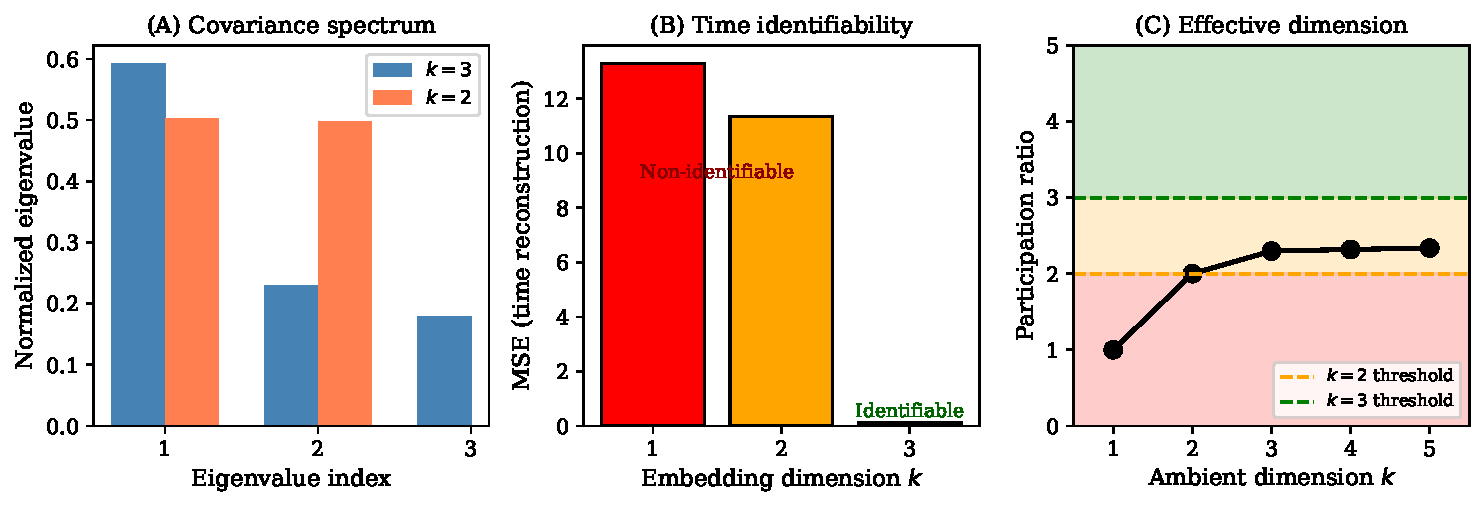
\includegraphics[width=\textwidth]{figures/fig2_fisher_rank.pdf}
    \caption{Information geometry of dimensional collapse. (A) Covariance spectrum for $k=3$ vs $k=2$ embeddings---the third eigenvalue is lost in projection. (B) Mean squared error in reconstructing meta-time from the embedded coordinates: reconstruction fails for $k \leq 2$ but succeeds for $k = 3$; shaded regions indicate regimes where $\tau$ is effectively non-identifiable (red) vs.\ identifiable (green). (C) Participation ratio (effective dimension) as a function of ambient dimension, showing the critical threshold at $k=3$.}
    \label{fig:fisher}
\end{figure}

Figure~\ref{fig:cycles} shows that the result generalizes to arbitrary directed cycles, not just simple 2-cycles.

\begin{figure}[htbp]
    \centering
    
\includegraphics[width=\textwidth]{figures/fig3_general_cycles.pdf}
    \caption{Generalization to directed cycles. (A) A 2-cycle (e.g., TRUE $\leftrightarrow$ FALSE oscillation) requires $k_{\min} = 3$. (B) A 3-cycle A $\to$ B $\to$ C $\to$ A also requires $k_{\min} = 3$. (C) More complex graphs with nested cycles similarly require $k \geq 3$ for self-intersection-free embedding.}
    \label{fig:cycles}
\end{figure}

\section{Discussion}

\subsection{Categorical vs.\ Continuous Representations}

Our results formalize a fundamental dichotomy in information processing, arising from the tension between \emph{recurrence} (repeating states) and \emph{progress} (monotone meta-time):

\begin{itemize}
    \item \textbf{Categorical regime ($k \leq 2$):} When a recurrent process is constrained to a bounded region in $\R^2$ (a limit cycle rather than an unbounded spiral), self-intersections become unavoidable. The phase-preserving constraint forces dimensional collapse of the trajectory cylinder $S^1 \times \R$ onto a circle $S^1$, obliterating the meta-time distinction. The system can only represent ``what'' state it is in, not ``when'' it occurred---a geometric bottleneck that naturally engenders discrete, symbolic representations.

    \item \textbf{Continuous regime ($k \geq 3$):} The extra degree of freedom allows the trajectory to spiral helically. The system can maintain strict recurrence in the projected phase plane $(x_1, x_2)$ while encoding progress in the transverse dimension $(x_3)$. This permits representations of processes that are simultaneously cyclic and temporally distinct.
\end{itemize}

This dichotomy suggests that the emergence of discrete symbols from continuous dynamics may be geometrically inevitable under dimensional constraints, particularly when the system is spatially confined (as in homeostatic biological systems that cannot drift unboundedly).

\begin{corollary}[Discretization as Quotient]\label{cor:quotient}
For a cyclic process with monotone meta-time, any $k \leq 2$ phase-preserving embedding induces a quotient map on the trajectory. Specifically, let $\sim$ denote the equivalence relation on $[0,T]$ defined by:
\[
t_1 \sim t_2 \iff \pi_k(\gamma(t_1)) = \pi_k(\gamma(t_2)).
\]
Then for $k \leq 2$, the equivalence classes $[t] = \{s : s \sim t\}$ are non-trivial (contain more than one element), and the induced map $\bar{\gamma}: [0,T]/{\sim} \to \R^k$ is well-defined.

The quotient space $[0,T]/{\sim}$ is the \emph{effective state space} of the collapsed representation. For cyclic processes, this quotient is homeomorphic to $S^1$: the meta-time information is ``quotiented out,'' leaving only the phase. Topologically, this corresponds to the bundle projection $\pi: S^1 \times \R \to S^1$ that fibers the trajectory over the cycle; the ``discretization'' is precisely the loss of the fiber coordinate.
\end{corollary}

\begin{remark}[Vertical Fibers and the Quotient Framework]\label{rem:fibers}
In the phase-preserving case $\pi_2|_K = f \circ \varphi|_K$, the equivalence relation $x \sim y \iff \pi_2(x) = \pi_2(y)$ has classes equal to the fibers of $\varphi$. Infinitesimally, the \emph{vertical} directions are those annihilated by $d\varphi$---precisely the meta-time directions. The collapse is a quotient by this vertical foliation. This provides the link to the companion paper on quotient geometry: in that framework, $\mathcal{V} = \ker(d\varphi)$ is the vertical distribution, $\mathcal{H} = \mathcal{V}^\perp$ is the horizontal distribution, and the Fisher metric degenerates along $\mathcal{V}$ after projection.
\end{remark}

\subsection{Connection to Dynamical Systems}

Our results resonate with classical results in dynamical systems theory, particularly the Poincar\'e-Bendixson theorem \citep{poincare1881memoire,bendixson1901courbes,guckenheimer1983nonlinear}, which states that continuous flows in $\R^2$ cannot exhibit chaotic behavior---only fixed points and limit cycles are possible. In $\R^3$ and higher, strange attractors and complex recurrent behavior become possible.

The parallel is suggestive: $k = 2$ naturally yields simple, categorical structure, while $k \geq 3$ \emph{can} support richer, process-oriented dynamics. Our contribution is to formalize this in an information-geometric setting.

\subsection{Applications}

While this paper focuses on the mathematical foundations, the results have potential applications in:

\begin{itemize}
    \item \textbf{Neural coding:} Understanding when neural representations must be discrete vs.\ continuous \citep{gallego2017neural}.
    \item \textbf{Machine learning:} Characterizing bottleneck dimensions in autoencoders and information bottleneck methods \citep{tishby2000information}.
    \item \textbf{Cognitive science:} As a speculative future direction, formalizing the emergence of symbolic thought from continuous neural dynamics.
\end{itemize}

These applications are left for future work.

\subsection{Open Questions}

Several mathematically precise questions remain:

\begin{enumerate}
    \item \textbf{Piecewise monotone meta-time:} What is $k_{\min}$ if $\tau$ is only \emph{piecewise} monotone (allowing reversals)? Conjecture: reversals that return to previously visited meta-times increase $k_{\min}$.

    \item \textbf{Noisy phase:} If the phase coordinate $\theta$ is only \emph{approximately} cyclic (subject to phase slips or noise), does the threshold remain at $k = 3$, or does it depend continuously on the noise magnitude?

    \item \textbf{Torus dynamics:} For processes on $S^1 \times S^1$ (two coupled phase oscillators with independent monotone meta-times), what is $k_{\min}$? The naive bound is $k_{\min} \leq 5$ (Whitney for 2-manifold), but the actual threshold may be lower.

    \item \textbf{Non-phase-preserving projections:} If the projection $\pi_k$ is allowed to \emph{distort} the phase structure (not just collapse the meta-time), can self-intersection-free embeddings exist in $\R^2$? What constraints on $\pi_k$ are necessary and sufficient?

    \item \textbf{Collision scaling:} For finite $\varepsilon > 0$, how does $|\mathcal{C}(\pi_2, \gamma)|$ scale with the number of cycles $n$ and the period $P$? Is there a universal scaling law?
\end{enumerate}

\section{Conclusion}

We have established that $k = 3$ is the minimal embedding dimension for self-intersection-free representation of cyclic processes with monotone meta-time on statistical manifolds. This result identifies a critical threshold in information geometry: below three dimensions, temporal information is necessarily lost when the cyclic structure is preserved, forcing categorical representations; at three dimensions and above, continuous processes can be faithfully represented.

The proofs are elementary, relying on the topology of the circle and the definition of injectivity, combined with the classical Whitney embedding principle. Yet the result has implications for understanding when and why discrete structures emerge from continuous substrates.

\section*{Statements and Declarations}

\textbf{Funding:} No external funding was received for this research.

\textbf{Competing Interests:} The author has no competing interests to declare.

\textbf{Data Availability:} All code for reproducing figures is available at \url{https://github.com/todd866/minimalembeddingdimension}.

\textbf{Use of AI Tools:} Large language models (Claude 4.5 Opus, Gemini 3 Pro, ChatGPT 5.1 Pro) were used to assist in the drafting of text and the generation of Python plotting code. The author bears full responsibility for the content of the work.

\bibliographystyle{unsrt}
\bibliography{references}

\end{document}
